\section{Transistorverstärker}

\subsection{Differenzstufen (Erweiterung)}

\subsubsection{Differenzstufe mit $\bm{I_{\rm BIAS}}$}

\begin{tabular}{ll}
    Differenz Eingangsspannungen:   & $V_D = V_{\rm B1} - V_{\rm B2}$       \\
    Differnz Ströme:                & $\diff I_C = I_{\rm C1} - I_{\rm C2}$
\end{tabular}

\vspace{0.2cm}
\textbf{Arbeitspunkt} für Differenzstufen meistens bei $V_{\rm B1} = V_{\rm B2}$

\vspace{0.2cm}

\begin{minipage}[c]{0.3\columnwidth}
    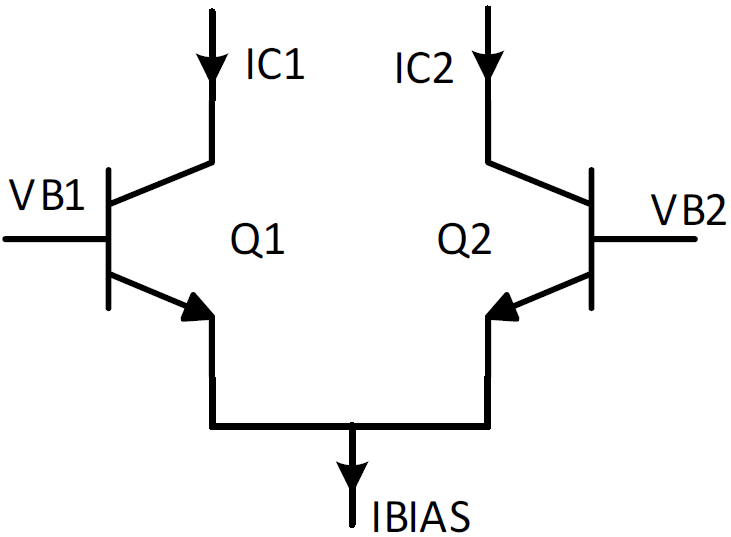
\includegraphics[width=\columnwidth]{images/differenzstufe_IBIAS.png}
\end{minipage}
\hfill
\begin{minipage}[c]{0.68\columnwidth}
    $$ \boxed{ \diff I_C(V_D) = I_{\rm BIAS} \cdot \tanh \Bigg( \frac{V_D}{2 \cdot n \cdot V_T} \Bigg) } $$
    $$ \boxed{ \frac{\diff I}{\diff V_{\rm in}} = I_{\rm BIAS} \cdot \frac{1 - \tanh \Big( \frac{V_D}{2 \cdot n \cdot V_T} \Big)^2 }{2 \cdot n \cdot V_T} } $$
\end{minipage}

\vspace{0.2cm}

$$ \boxed{ gm =  \frac{\diff I_C(V_D)}{\diff V_D} = \frac{I_{\rm BIAS}}{2 \cdot n \cdot V_T}  \cdot \Bigg( 1 - \tanh \Big( \frac{V_D}{2 \cdot n \cdot V_T} \Big)^2 \Bigg) } $$
$$ \boxed{ \text{Für } V_D = 0: \;  gm_{\rm DiffStufe} = \frac{I_{\rm BIAS}}{2 \cdot n \cdot V_T} } $$


\subsubsection{Differenzverstärker}

\begin{minipage}[c]{0.48\columnwidth}
    $$ \Delta V_{\rm in} = V_{\rm in1} - V_{\rm in2} $$
\end{minipage}
\hfill
\begin{minipage}[c]{0.48\columnwidth}
    $$ \Delta V_{\rm out} = V_{\rm out1} - V_{\rm out2} $$
\end{minipage}

\vspace{0.2cm}

\begin{minipage}[c]{0.35\columnwidth}
    \begin{center}
        \myul{\textbf{Schaltung}}

        \vspace{0.2cm}

        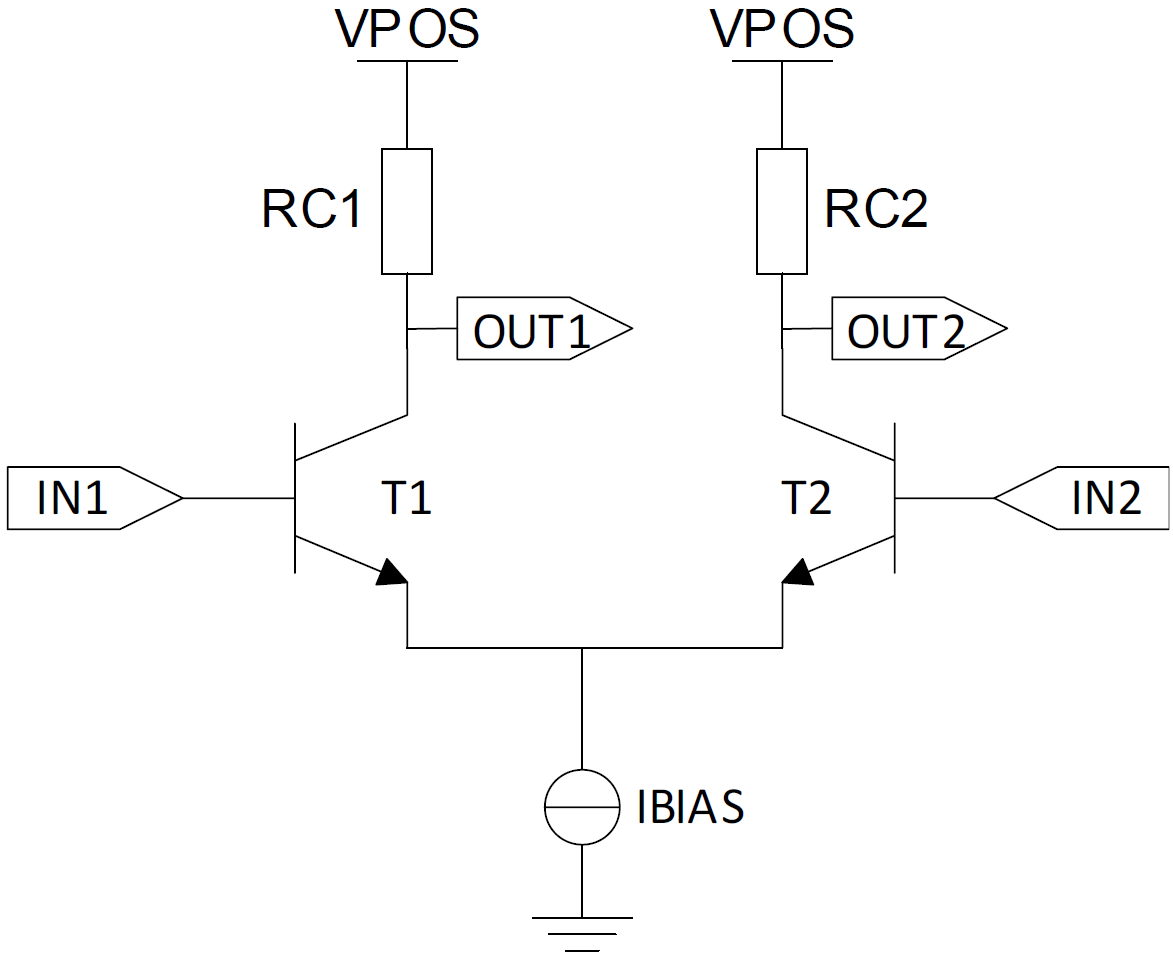
\includegraphics[width=\columnwidth]{images/differenzstufe_kollektorwiderstand.png}
    \end{center}
\end{minipage}
\hfill
\begin{minipage}[c]{0.55\columnwidth}
    \begin{center}
        \myul{\textbf{Kleinsignal-Ersatzschaltung}}

        \vspace{0.2cm}

        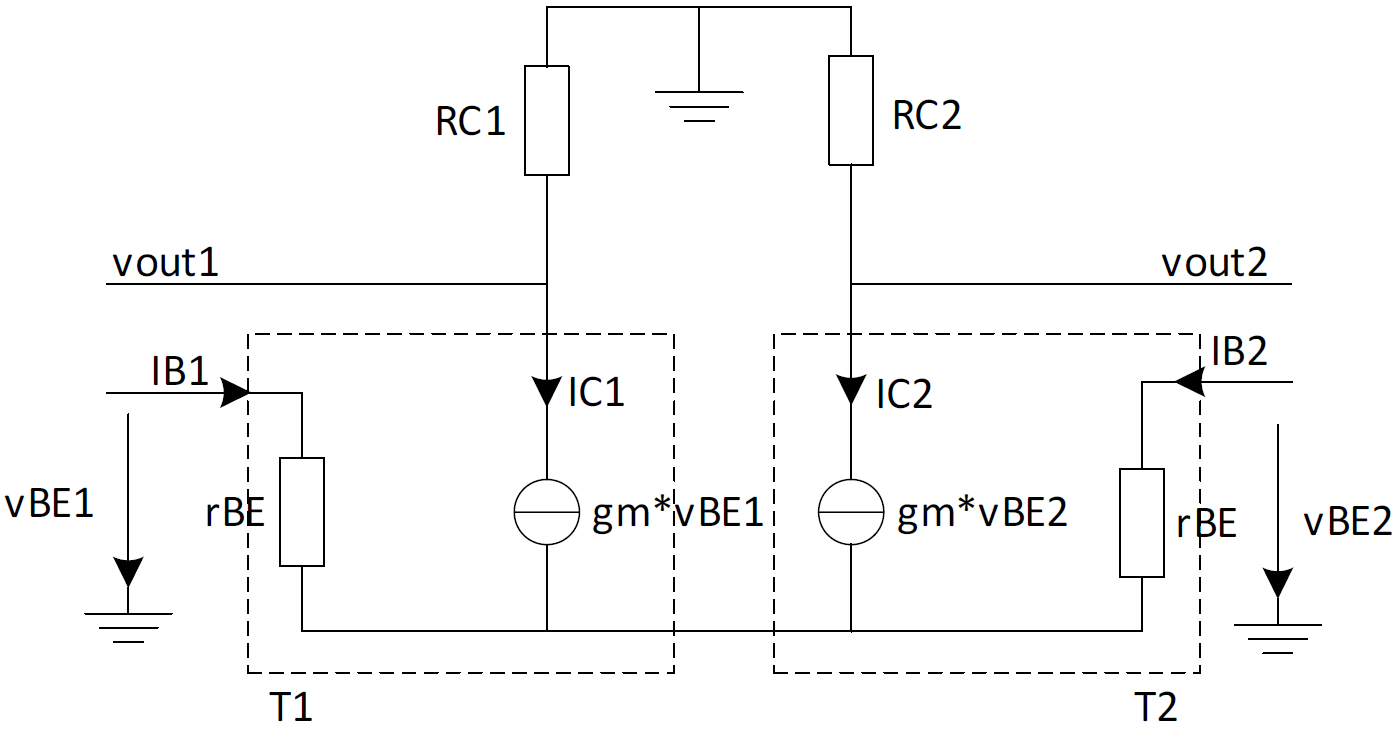
\includegraphics[width=\columnwidth]{images/differenzstufe_kollektorwiderstand_kleinsignalersatzschlatung.png}
    \end{center}
\end{minipage}

\vspace{0.2cm}

\begin{itemize}
    \item Arbeitspunkt bei $ V_{\rm in1} = V_{\rm in2} $
    \item $\frac{I_{\rm BIAS}}{2}$ fliesst durch $T_1$ bzw. $T_2$
    \item Aus Kleinsignalersatzschaltung: $I_{\rm C2} + I_{\rm B2} = - (I_{\rm C1} + I_{\rm B1})$
    \item $v_{\rm BE1} = \frac{\Delta V_{\rm in}}{2}$ und $v_{\rm BE2} = - \frac{\Delta V_{\rm in}}{2}$
\end{itemize}


$$ \boxed{ gm = \frac{\diff I_{\rm C1}}{\diff V_{\rm BE1}} = \frac{I_{\rm C1}}{n \cdot V_T} = \frac{I_{\rm BIAS}}{2 \cdot n \cdot V_T} } \quad \boxed{ r_{\rm BE} = \frac{2 \cdot \beta \cdot n \cdot V_T}{I_{\rm BIAS}} } $$
$$ \boxed{ \Delta V_{\rm out1} = - \frac{1}{2} \Delta V_{\rm in} \cdot gm \cdot R_{\rm C1} } \quad \boxed{ \Delta V_{\rm out2} = \frac{1}{2} \Delta V_{\rm in} \cdot gm \cdot R_{\rm C2} } $$
$$ \boxed{ \text{Verstärkung: } A = \frac{\Delta V_{\rm out}}{\Delta V_{\rm in}} = - gm \cdot R_C = - \frac{I_{\rm BIAS}}{2 \cdot n \cdot V_T} \, R_C } $$ 


\subsubsection{Differenzstufe mit Emitterfolger}

\begin{minipage}[c]{0.35\columnwidth}
    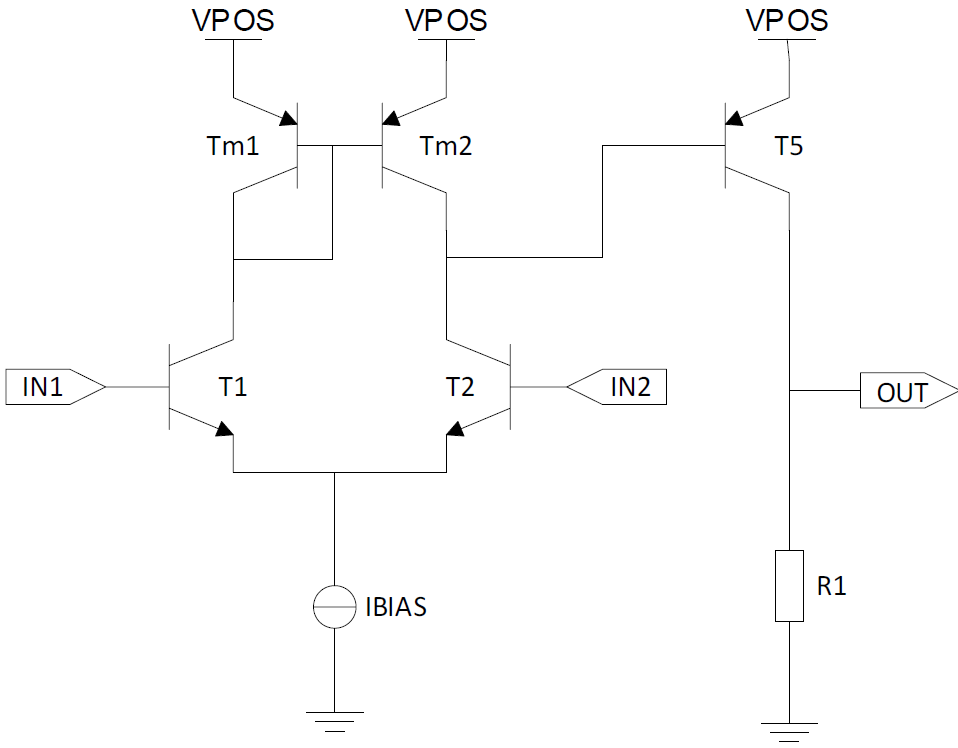
\includegraphics[width=\columnwidth]{images/differenzstufe_emitterfolger.png}
\end{minipage}
\hfill
\begin{minipage}[c]{0.55\columnwidth}
    \raggedright

    \begin{itemize}
        \item $I_{\rm out}$ von Diff-Stufe wird von $T_5$ mit Faktor $\beta$ verstärkt
        \item $R_1$ wandelt Strom in Spannung
    \end{itemize}

    \vspace{0.2cm}

    $$ \boxed{ A = \frac{\Delta V_{\rm out}}{\Delta V_{\rm in}} = \beta \cdot R_1 \cdot \frac{I_{\rm BIAS}}{2 \cdot n \cdot V_T} } $$
\end{minipage}


\subsubsection{Differenzverstärker mit Stromspiegel-Last (OTA)}

\begin{minipage}[c]{0.35\columnwidth}
    \begin{center}
        \myul{\textbf{Schaltung}}

        \vspace{0.2cm}

        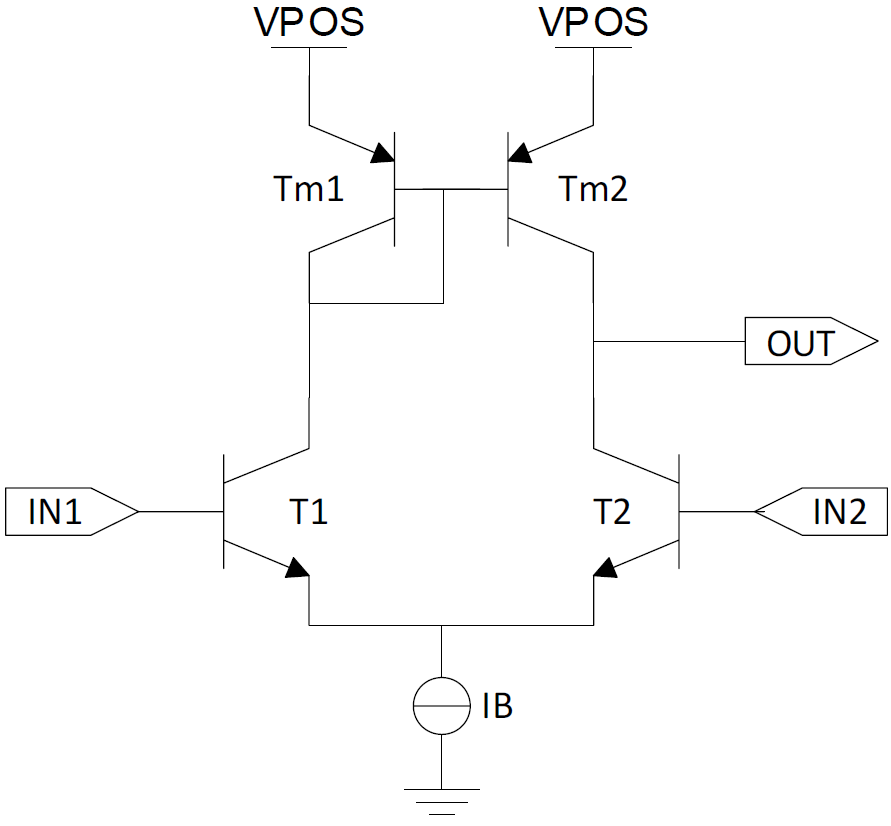
\includegraphics[width=\columnwidth]{images/differenzverstaerker_stromspiegel.png} 
    \end{center}
\end{minipage}
\hfill
\begin{minipage}[c]{0.55\columnwidth}
    \begin{center}
        \myul{\textbf{Kleinsignal-Ersatzschaltung}}

        \vspace{0.2cm}

        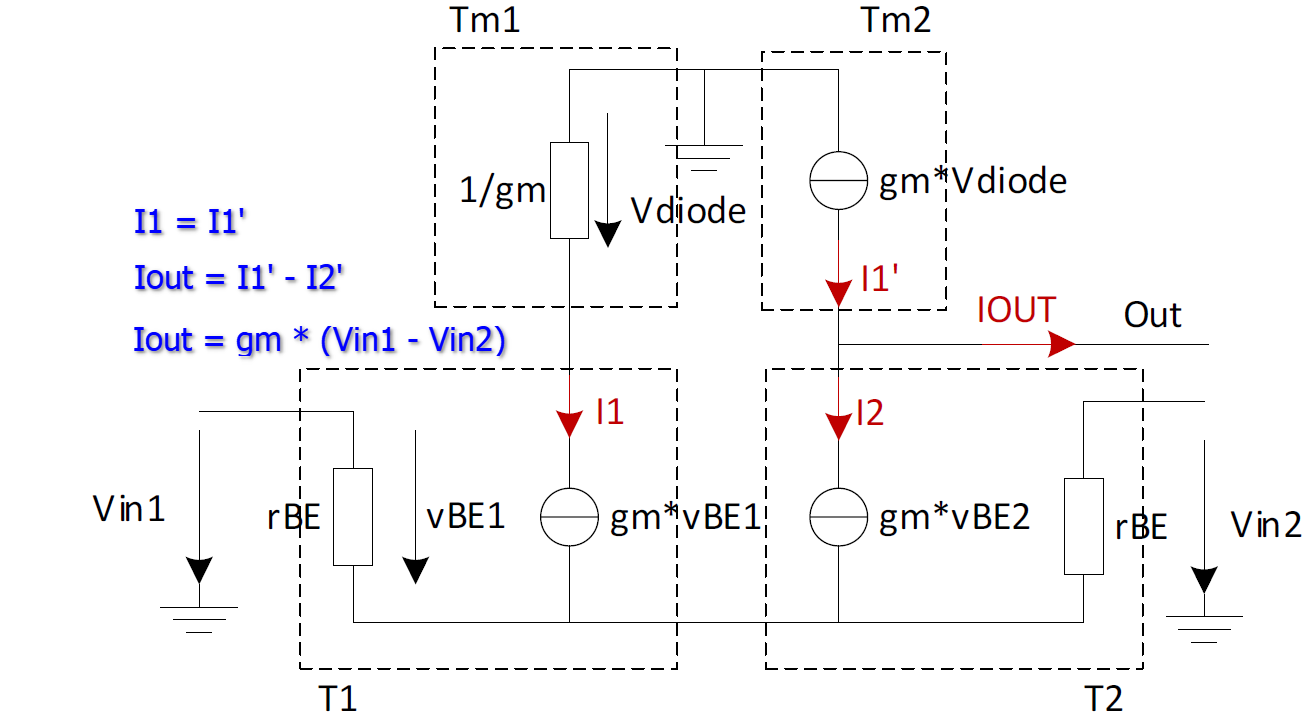
\includegraphics[width=\columnwidth]{images/differnzverstaerker_stromspiegel_ersatzschaltung.png} 
    \end{center}
\end{minipage}

\vspace{0.2cm}

\begin{itemize}
    \item Hoher Ausgangswiderstand $r_{\rm out} = r_{\rm CE1} || r_{\rm CE2}$
    \item Minimale Eingangsspannung: $\approx 0.9 \, \volt$
    \item Maximale Eingangsspannung: $V_{\rm POS} - V_{\rm CE,sat}$
\end{itemize}

$$ \boxed{ gm = \frac{I_{\rm BIAS}}{2 \cdot n \cdot V_T} } \quad \boxed{ I_{\rm out} = gm \cdot (V_{\rm in1} - V_{\rm in2}) = \frac{I_{\rm BIAS}}{2 \cdot n \cdot V_T} \cdot \Delta V_{\rm in} } $$ 


\subsubsection{Differenzstrufe mit Stromquelle}

\begin{minipage}[c]{0.4\columnwidth}
    \begin{center}
        \myul{\textbf{Hochohmige Lasten}}

        \vspace{0.2cm}

        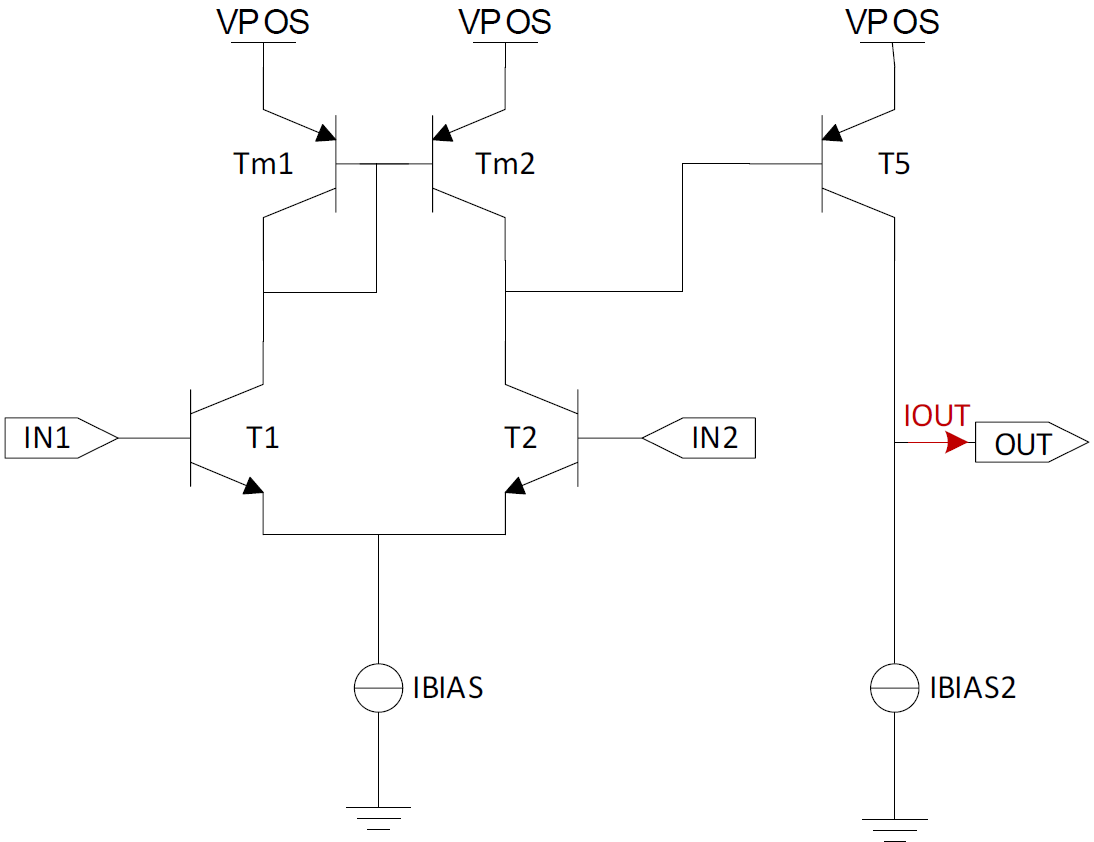
\includegraphics[width=\columnwidth]{images/differenzstufe_stomquelle_hochohmig.png}

        $$ \boxed{ I_{\rm out} = \beta \cdot \frac{I_{\rm BIAS}}{2 \cdot n \cdot V_T} \cdot \Delta V_{\rm in} } $$
    \end{center}    
\end{minipage}
\hfill
\begin{minipage}[c]{0.4\columnwidth}
    \begin{center}
        \myul{\textbf{Niederohmige Lasten}}

        \vspace{0.2cm}

        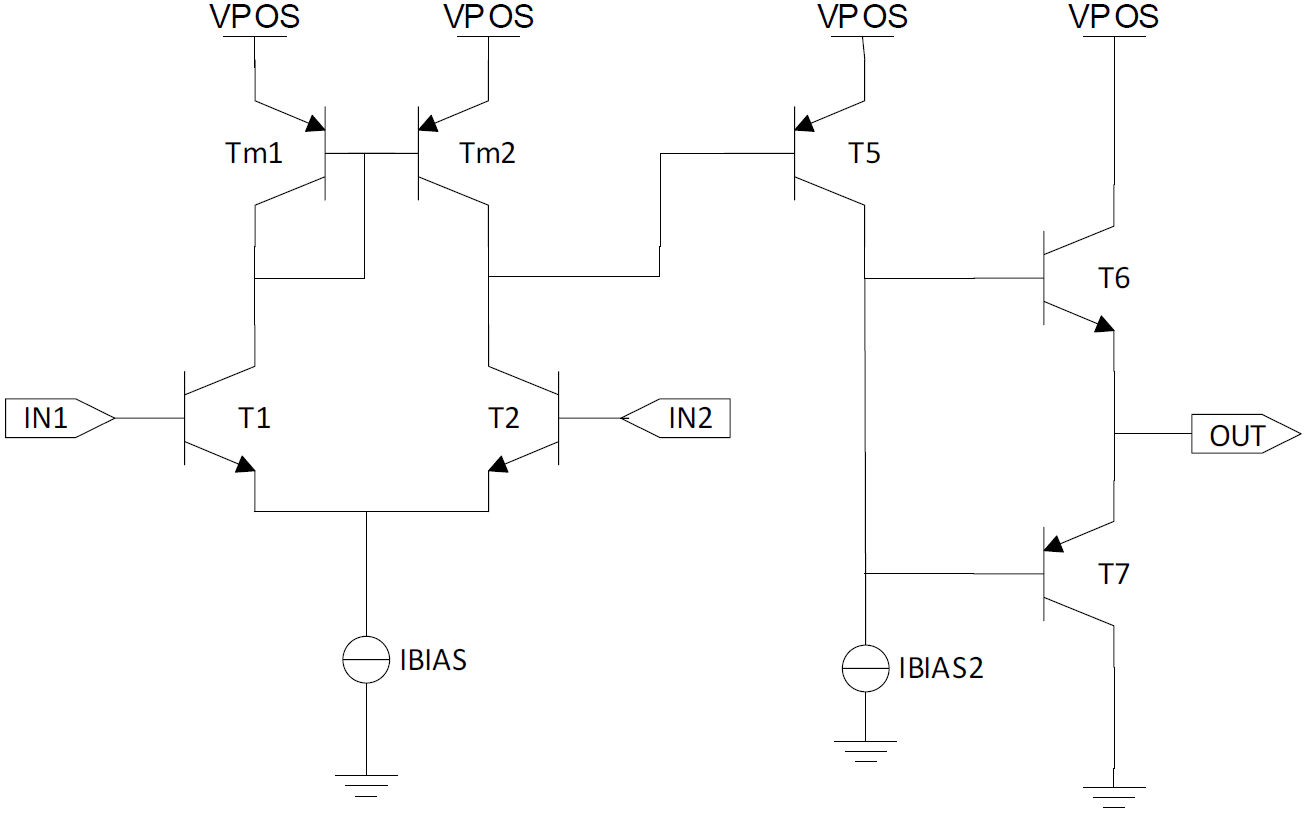
\includegraphics[width=\columnwidth]{images/differenzstufe_stomquelle_niederohmig.png}

        \vspace{0.2cm}

        OTA ergänzt mit Class-B Buffer
    \end{center}
\end{minipage}


\subsubsection{Differenzstufe mit Emitterfolger und Class-AB Buffer}

\begin{minipage}[c]{0.43\columnwidth}
    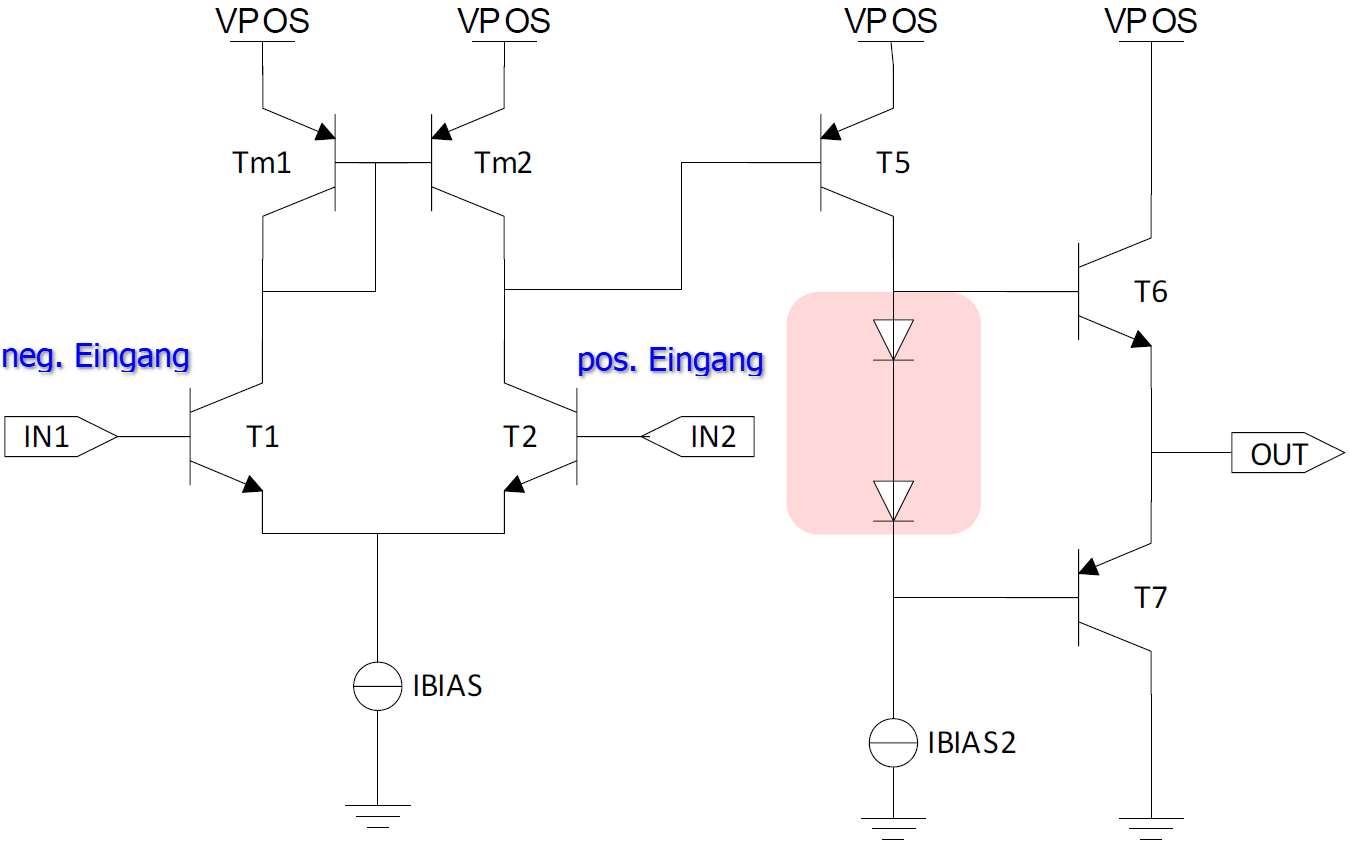
\includegraphics[width=\columnwidth]{images/differenzstufe_emitterfolger_buffer.png} 
\end{minipage}
\hfill
\begin{minipage}[c]{0.53\columnwidth}
    \raggedright

    \begin{itemize}
        \item Erlaubt Verstärkungen $\geq 10'000$
        \item \textbf{Schaltung ist 'Komparator'oder Verstärker mit Rückkopplung auf neg. Eingang}
    \end{itemize}
\end{minipage}


\subsection{Darlington-Schaltung}

Darlington-Schaltungen werden eingesetzt, um grössere Stromverstärkungen zu erzielen.


\subsubsection{Darlington}

\begin{minipage}[c]{0.16\columnwidth}
    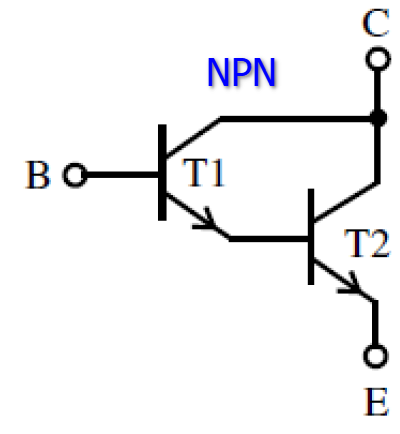
\includegraphics[width=\columnwidth]{images/darlington_npn.png} 
\end{minipage}
\hfill
\begin{minipage}[c]{0.16\columnwidth}
    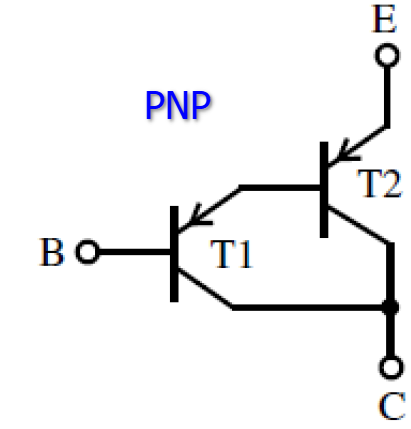
\includegraphics[width=\columnwidth]{images/darlington_pnp.png} 
\end{minipage}
\hfill
\begin{minipage}[c]{0.58\columnwidth}
    $$ \boxed{ V_{\rm BE} = V_{\rm BE1} + V_{\rm BE2} } $$
    $$ \boxed{ \beta = \beta_1 + \beta_2 } $$
\end{minipage}


\subsubsection{Komplementär-Darlington}

\begin{minipage}[c]{0.22\columnwidth}
    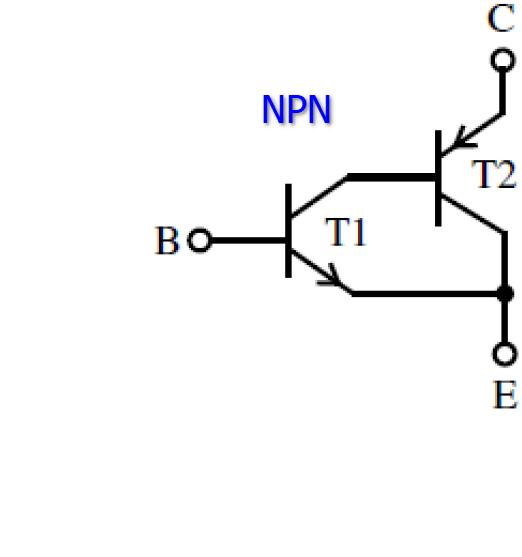
\includegraphics[width=\columnwidth]{images/komplementaer_darington_npn.png} 
\end{minipage}
\hfill
\begin{minipage}[c]{0.22\columnwidth}
    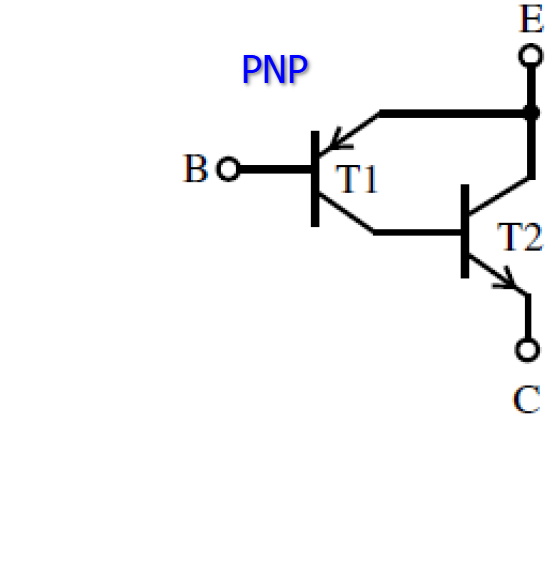
\includegraphics[width=\columnwidth]{images/komplementaer_darington_pnp.png} 
\end{minipage}
\hfill
\begin{minipage}[c]{0.48\columnwidth}
    $$ \boxed{ V_{\rm BE} = V_{\rm BE1} } $$
    $$ \boxed{ \beta = \beta_1 + \beta_2 } $$
\end{minipage}

\vspace{-0.4cm}


\subsection{Verstärker mit Current Feedback OpAmp}

\begin{minipage}[c]{0.32\columnwidth}
    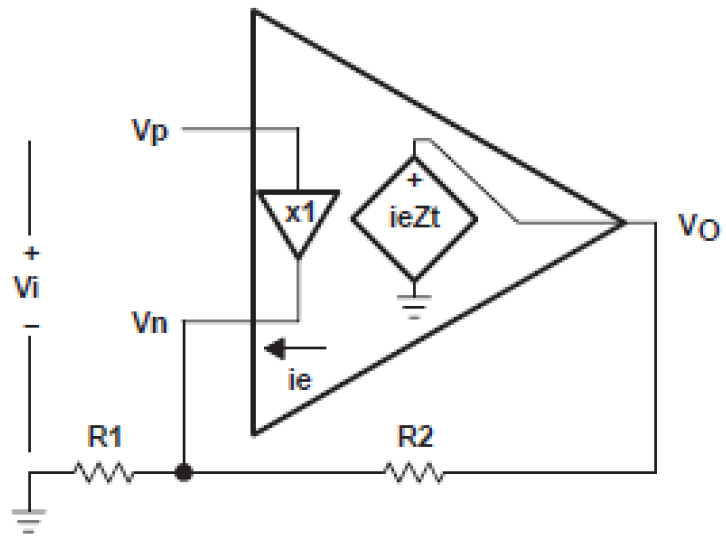
\includegraphics[width=\columnwidth]{images/verstaerker_current_feedback_opv.png} 
\end{minipage}
\hfill
\begin{minipage}[c]{0.63\columnwidth}
    \raggedright

    \begin{itemize}
        \item $Z_t = $ sehr grosse interne Impedanz
        \item $I_e$ regelt sich über Feedback auf 0
        \item Verstärkung wie normaler OpAmp aber viel schneller
    \end{itemize}

    $$ \boxed{ V_p = V_n = V_o \frac{R_1}{R_1 + R_2} } \quad \boxed{ V_o = V_p \, \Bigg( 1 + \frac{R_2}{R_1} \Bigg) } $$
\end{minipage}

